\subsection{Feature extraction}

% Use 'Linear and non linear regression techniques for Simultaneus and prop...' + 'Feature reduction and selection for EMG signal classification'

%HEAD
%The following section will feature feature extracion, 

Following preprocessing of the recorded EMG signal, features can be extracted and used to map different hand gestures. Features are extracted from the signal to represent the signal using fewer data samples. This is also called dimension reduction and result in faster computation times. When analyzing EMG signals there will be three different signal components to be extracted, which are the frequency and time domains, as well as the time-scale representation. Frequency domain features require a Fourier transformation of the signal, which requires more processing than the direct extraction of time domain features. \cite{phiny2012} \\
%In order to extract the features which can be used to differ between the movements performed by the wearer, different features can  extraction can be implemented. In addition to highlighting important features within the signal, the implementation of feature extraction will be useful when it comes to removing unwanted signal features caused by noise sources such as the powergrid and movement of the electrodes. \cite{phiny2012}
The time domain features are extracted directly from the EMG signal, and these feature extraction methods are often used both for research and practices since they often require very little processing compared to frequency domain features. Time domain features are mainly focused on the amplitude of the signal, which means they have a disadvantage if the signal differs in amplitude due to muscle fatigue. \cite{phiny2012} Different features are visualized in \figref{fig:EMGfeatures}. 

\begin{figure}[H]                    
	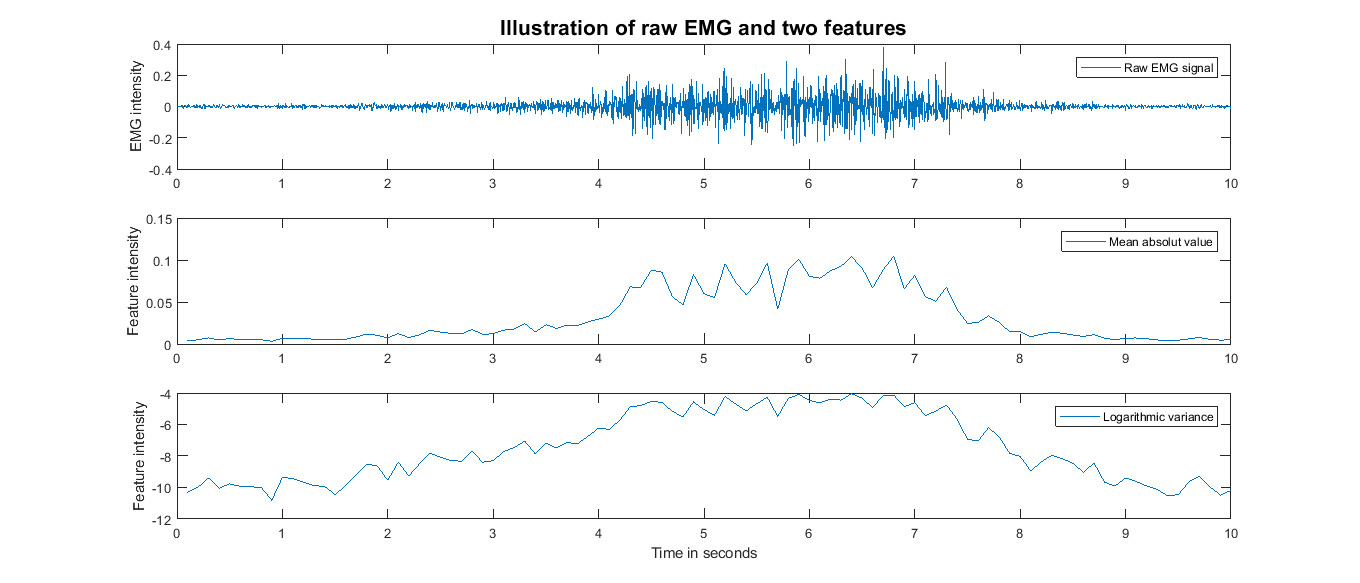
\includegraphics[width=1\textwidth]{figures/background/EMG_features}  %<--but is not needed.
	\caption{Above a raw EMG signal. Below are different features extracted from the EMG signal presented.}
	\label{fig:EMGfeatures}
\end{figure}

%Based on the study af Hahne et al. \cite{hahne2014}, we will choose logarithmic variance as the feature to be extracted from the recorded EMG signal. Hahne et al. finds that the cross-validation performance improves significantly with the use of linear regression combined with logarithmic variance, compared to combining the linear regression with variance or RMS. \cite{hahne2014}. 

%Choice of feature will be based on previous studies of performance of different extracted features. 
%%, where the method will be chosen based on it's performance in the low frequency area and the processing time for the feature to be extracted. 
%This is a result of the Myo armband limiting the recordable signal to 100 Hz, and the intend of being able to control the JACO arm in real-time, where a long processing time would cause a delay between hand movement and movement of the JACO arm.
%This study will only implement time domain features, due to the low sampling rate of the Myo band, which means that an implementation of frequency domain features will not be useful, as the signal does not contain a lot of information in that domain. The feature chosen in this study will be the logarithmic variance of the signal, based on a previous study by \cite{hahne2014}, where they find that this feature is useful for methods based on the numerical range of the features. \cite{hahne2014} 